\documentclass[defaultstyle,11pt]{thesis}

\usepackage{amsmath} % assumes amsmath package installed    
\usepackage{amssymb}  % assumes amsmath package installed
\usepackage{url}
\usepackage{float}
\usepackage{graphicx}
\usepackage{algorithm,algpseudocode}
\usepackage{subcaption}
\usepackage{stfloats}
\usepackage{booktabs}
\usepackage{multirow}

\title{PMorph: A Task-Specialized Robot Manipulator Morphology Optimizer}

\author{Stephen}{Gillet}

\otherdegrees{B.S., Texas Tech University, 2023}

\degree{Master of Science}		%  #1 {long descr.}
	{M.S., Robotics}		%  #2 {short descr.}

\dept{Department of}			%  #1 {designation}
	{Robotics}		%  #2 {name}

\advisor{Prof.}				%  #1 {title}
	{Alessandro Roncone}			%  #2 {name}

\reader{Sean Humbert}		%  2nd person to sign thesis
\readerThree{Leopold Beuken}		%  3rd person to sign thesis

\abstract{    \OnePageChapter
    This paper seeks to address the energy-ineffiency, lack of task specialization, and overactuation seen in manufacturing from the current suite of generalized robotic manipulators.
    The approach involves specifying a task in a MuJoCo simulated environment and then using a PPO agent to optimize the morphology for that enviroment given a reward function.
    The morphological elements to be optimized include the number of links, the lengths of each link, and the type of joints involved.
    The reward function is tuned to weigh energy cost, end effector movement, end effector accuracy, manipulability measures, number of links, and task completion.
    PPO is ideal for this task because it can efficiently optimize over the continuous action space that is morphology, resulting in a robot that is more simple, efficient, and capable than those commonly used in industry today. 
}

\acknowledgements{   \OnePageChapter
    My advisor Dr. Alessandro Roncone and my mentor Gilberto Briscoe-Martinez deserve credit for generating and refining the idea and helping me to refine the process along the way and pushing me to attempt and learn more than I would have on my own.
    Credit should also go to the other members of the HIRO lab for helping me brainstorm and to my support system: my family, the Alano Club of Boulder, and my dear friend Donnie Prante who give me life advice and perspective.
}

\LoTisShort

\begin{document}


%%%%%%%%%%%%%%%%%%%%%%%%%%%%%%%%%%%%%%%%%%%%%%%%%%%%%%%%%%%%%%%%%%%%%%%%%%%%%%%%

%%%%%%%%%%%%%%%%%%%%%%%%%%%%%%%%%%%%%%%%%%%%%%%%%%%%%%%%%%%%%%%%%%%%%%%%%%%%%%%%
\chapter{Introduction}

\begin{figure*}[!b] % [!b] forces it to the bottom, stfloats allows it on page 1
    \centering
    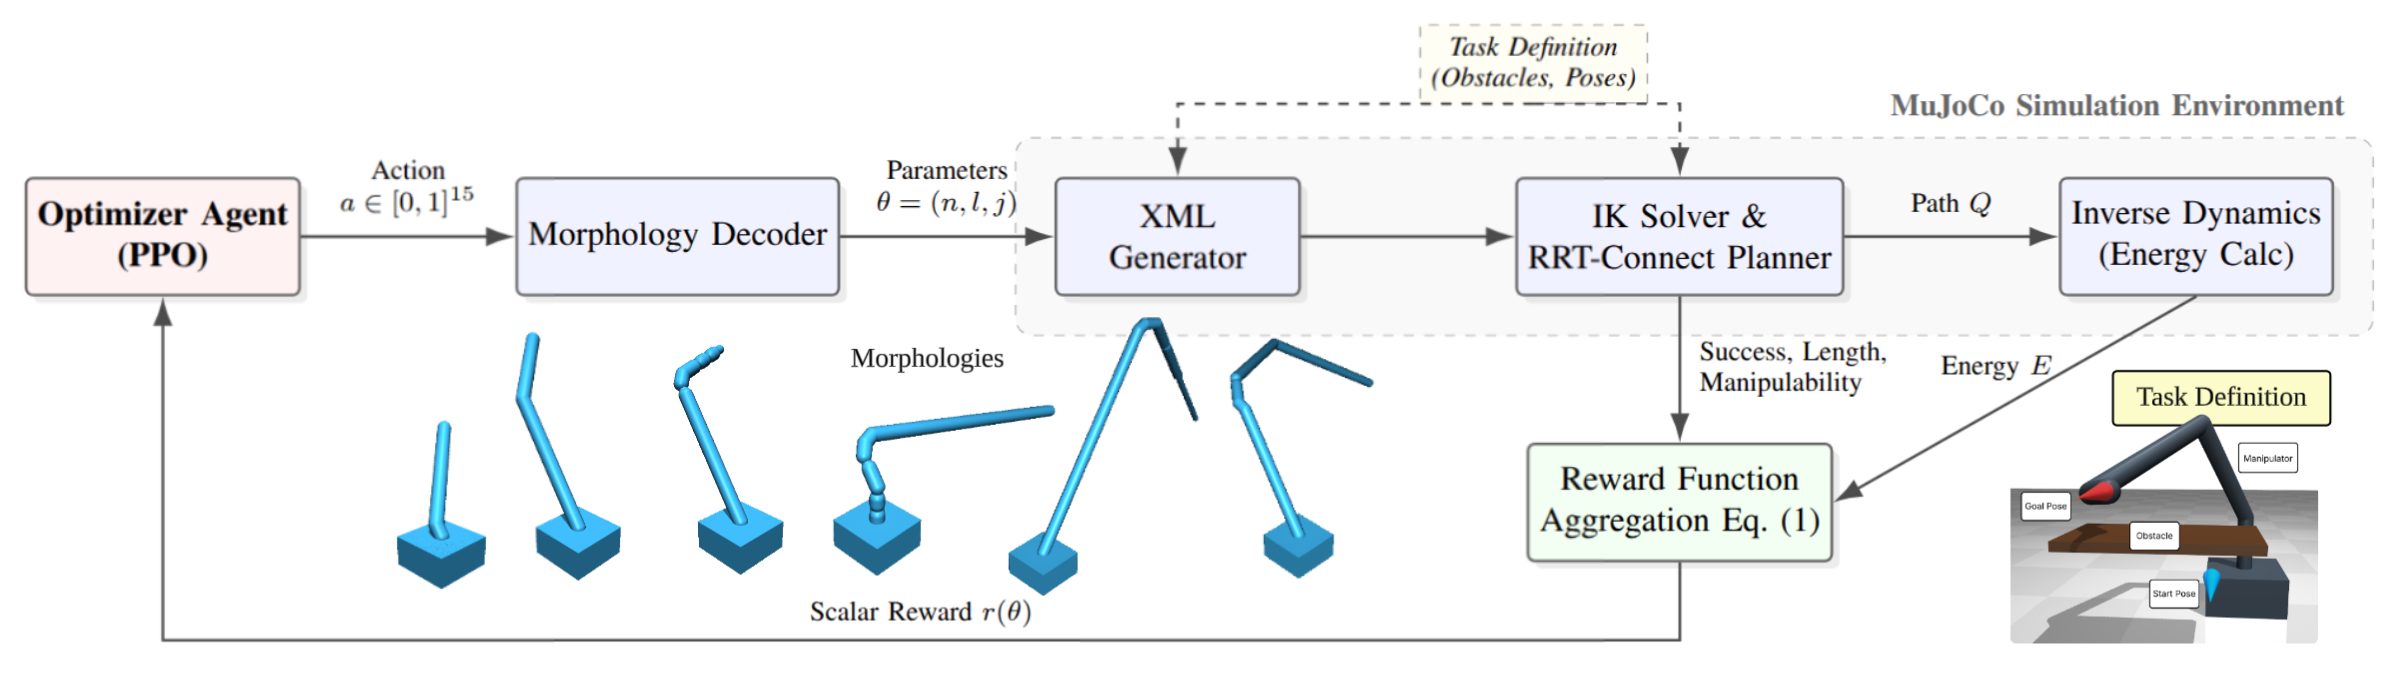
\includegraphics[width=\textwidth]{systemDiagram.png}
    \caption{System overview of the proposed morphology optimization framework. The optimizer agent generates actions \( a \in [0,1]^{15} \), which are decoded into robot parameters \( \theta = (n, l, j) \) (number of links, lengths, and joint types). These are used to create an XML model evaluated in a MuJoCo simulation environment, incorporating task definitions (obstacles and start/goal poses). IK solving and RRT-Connect path planning compute trajectories \( Q \), followed by inverse dynamics for energy \( E \). Performance metrics (success, path length, manipulability, and energy) are aggregated via the reward function in Eq. (1) to yield a scalar reward \( r(\theta) \).}
    \label{fig:systemDiagram}
\end{figure*}

Imagine a factory where every employee has to be trained on and work every job in the plant.
Research (\cite{staats2012specialization}\cite{madiedo2020capturing}) shows that approach to be inefficient because workers cannot build deep expertise and become very productive.
The majority of factories today use specialized workers for this reason, dividing tasks boosts efficiency, reduces costs, and increases output \cite{jackson2025story}\cite{indeed2025pros}. 
And yet, this is exactly the opposite approach of robotics in manufacturing today where high costs and lack of tailorability are some of the most cited problems for the adoption of robotics \cite{mckinsey2019industrial}\cite{patel2024}.
To make matters worse \cite{russo2021task} and \cite{he2019underactuated} show that most robot manipulators are overactuated, inefficient, and ineffective for most tasks they are used in today.

What if, in the same way that factories do with human workers, robots were specialized in the tasks they performed?
Much like human workers physically and cognitively adapt to master repetitive tasks over time \cite{arany2008pgc1}\cite{mancuso2022effect}\cite{wu2020occupational}, robotic systems stand to gain significant efficiencies through morphological specialization. 
As advancements in additive manufacturing and Industry 4.0 drive the cost of mass customization closer to that of traditional mass production \cite{wang2017industry}\cite{baumers2019economics}, it is becoming both economically feasible and operationally necessary to co-optimize a robot's physical hardware alongside its control software for specific workspaces.
This paper seeks to optimize the morphological design of robots to specific tasks by using a PPO agent to optimize the morphology based on various performance metrics and task-specific physical constraints.
This ensures that the robot is as simple, efficient, and capable as possible for its particular job while still allowing the designer to specify the level of robustness.

PPO was chosen for its ability to explore the continuous action space that is morphology and it has been shown to do so efficiently and robustly \cite{schulman2017proximal}.
The core method is to use Stable Baselines3 PPO implementation to iterate on the design parameters (number of links, joint types (X, Y, Z hinge, and Z actuation), and link lengths), use MuJoCo to simulate that iteration on a simple task using a simple controller (RRT-Connect and damped least squares (DLS) inverse kinematics (IK) for path planning), and feed the results (success, efficiency, and manipulability index) back into the PPO model.
OMPL's RRT-Connect was chosen for simplicity and it has been shown to be faster than other methods \cite{kuffner2000rrt,sucan2012ompl} which enables faster and more robust training.
DLS IK was chosen for a similar reason, it has been shown to be robust especially in situations where the target position is out of reach \cite{buss2004introduction} which is inevitable when exploring morphologies, some of which will be too small or otherwise poorly suited to the task as the agent learns.

The evaluation signals will be successful path planning, path length, energy cost, and manipulability index.
The manipulability index is a measure of a manipulators ability to arbitrarily change the position and orientation of the end effector at a particular point, borrowed from \cite{yoshikawa1985manipulability}.
The tasks will be kept simple but varied in ways to test different types of movements like moving near the base, moving from near to far, different elevations, more linear movements, and different obstacle contraints.
One might imagine that a lot of pick and place tasks are mostly linear and so might largely be done by linear actuators more efficiently for example.

The research questions to be answered: 
\begin{enumerate}
    \item Can PPO be used to generate more efficient morphologies?
    \item Can morphologies be generated for tasks that generalized manipulators cannot do or cannot perform well?
    \item Can more simple morphologies (less DOF) be generated that can perform the same tasks with similar levels of accuracy?
\end{enumerate}

\chapter{Related Work}

While most of the work in this area has focused on the co-optimization of morphology and control for atomic, modular robots, AI has been increasingly shown to aid in the design of efficient robotics.
This section dives into the background research specifically pertaining to the three research questions: energy efficiency, task specialization, and simplicity in manipulator design.
Can PPO be used to do it?

\section{Energy Efficiency}
One of the primary motivations for morphology optimization is energy efficiency.
Recent literature has shown that the traditional approach of optimizing controllers for energy efficiency can be significantly augmented by optimizing the morphology itself.
\cite{bhatia2023reinforcement} shows that PPO can be used to generate freeform morphologies from atomic modules for efficient gaits.
\cite{luck2019data} shows that Soft Actor Critic (SAC) can also be used to create more efficient gaits, this time by codesigning morphology and control on quadrapeds.
\cite{le2020reinforcement} uses RL to do path planning for modular, reconfigurable, tiling robots that includes morphology configuration and is more energy efficient than conventional methods.
This work provides the motivation to use PPO to optimize morphology for energy efficiency.

\section{Task Specialization}
Basic manipulators often struggle in highly constrained or atypical environment which prompts research into task-specific morphology design.
\cite{kalimuthu2023} demonstrates the effectiveness of PPO and A3C at generating configurations for reconfigurable tiling robots to maximize coverage in specialized environments.
\cite{ding2024modular} proves that DDQN can be used to generate morphologies and controllers for reconfigurable robots in order to do tasks that fixed morphologies cannot or cannot perform well.
\cite{spielberg2025accelerated} did the same thing with the addition of a foundation model to speed training and increase effectiveness.
PMorph builds on this by using obstacle and task-aware morphology optimization to design around morphology weaknesses that basic arms would fall into.

\section{Simplicity}
FANUC 6-DOF series of manipulators are the most commonly used in industry today \cite{patentpc2025toprobotics}\cite{standardbots2025fanucprice} and the 7-DOF Franka Emika Panda is considered a standard in research \cite{haddadin2022franka}\cite{oliva2022franksim}.
However, \cite{russo2021task} and \cite{he2019underactuated} indicate that these common, general-purpose manipulators are overactuated for most of the tasks they are used in leading to parasitic mass and computational waste.
\cite{fasquell2020bioinspired} and \cite{nakano2023robostrich} show that reduced DOF designs can be efficient and effective.
PMorph addresses simplicity directly by having a reward term that can be used to punish additional DOF, allowing optimization for accuracy and simplicity at the same time.

\chapter{Problem Formulation}
\label{sec:problem}

The task is formulated as a single-step reinforcement learning problem in a MuJoCo simulated environment.
A morphology $\theta$ is chosen, run through the simulation, and then evaluated based on weighted reward function terms.

\section{Morphology Parameterization}

A candidate morphology is defined by the tuple
\[
\theta = (n, l, j),
\]
where
\begin{itemize}
    \item $n \in \{2, \dots, 7\}$ is the number of links,
    \item $l = [l_1, \dots, l_n] \in [0.05, 1.2]^n$ are the link lengths (m),
    \item $j = [j_1, \dots, j_n] \in \{0,1,2,3\}^n$ are the joint types (0: revolute about x, 1: about y, 2: about z, 3: slide in z).
\end{itemize}
The action space of the RL agent is the continuous box
\[
\mathcal{A} = [0,1]^{1 + 7 + 7},
\]
from which $n$, $l$, and $j$ are decoded.

\section{Task Specification}

The robot has to move from start poses to goal poses (position + unit quaternion) in a cluttered workspace with fixed obstacles (walls, shelves, ceilings).
An example of such an environment may be seen in Figure \ref{fig:containerTask}, which shows the container task where two sets of start and goal poses are set at either ends of a shipping-container-like workspace with the arm positioned in the middle.
The poses are modified with Gaussian noise ($\sigma=0.05$) at evaluation in order to encourage robust designs.

\begin{figure}[H]
    \centering
    \begin{subfigure}[b]{0.45\columnwidth}
        \centering
        
\includegraphics[width=\textwidth]{containerTask1.png}
        \caption{Task 1: Deep Extraction}
        \label{fig:container_1}
    \end{subfigure}
    \begin{subfigure}[b]{0.45\columnwidth}
        \centering
        
\includegraphics[width=\textwidth]{containerTask2.png}
        \caption{Task 2: Shallow Extraction}
        \label{fig:container_2}
    \end{subfigure}
    \caption{\textbf{Container task evaluation.} The manipulator is tasked with reaching deep into a constrained, container-like environment (start poses in blue) and extracting to an open area (goal poses in red). This highly constrained task tests the morphology's compactness and ability to perform high-reach tasks without colliding with ceiling or wall constraints.}
    \label{fig:containerTask}
\end{figure}

\section{Evaluation Pipeline}

Morphology $\theta$ is evaluated as follows:
\begin{enumerate}
    \item A MuJoCo XML model is generated with $\theta$ and the task poses/obstacles.
    \item Inverse Kinematics is solved for the start and goal poses using Damped Least Squares.
    \item A path between the start and goal configurations is computed using RRT-Connect.
    \item If a path connect be found, return reward $30 - 100 \times \text{IK error}$.
    \item Otherwise, calculate the other reward terms and return the weighted sum:
    \begin{itemize}
        \item End-effector path length $p = \sum \|\mathbf{x}_{ee}^{t+1} - \mathbf{x}_{ee}^t\|$ (Euclidean distance between each point along path),
        \item Manipulability $\mu = \min(\sigma(\mathbf{J}))$ (minimum singular value of manipulability jacobian at start and goal \cite{klein1987dexterity}),
        \item Energy $E = \sum \|\boldsymbol{\tau} \odot \mathbf{v}\| \cdot \Delta t$ (MuJoCo inverse dynamics using constant velocity segments along path at torque limits).
    \end{itemize}
\end{enumerate}

\section{Reward Function}

The scalar reward is
\begin{align}
r(\theta) &= \frac{1}{N} \sum_{i=1}^{N} \Biggl[ 
    w_0 \cdot \text{success}_i 
    - w_1 \cdot p_i \notag \\
    &\quad - w_2 \cdot (e_{\text{start},i} + e_{\text{goal},i}) 
    + w_3 \cdot (\mu_{\text{start},i} + \mu_{\text{goal},i}) \notag \\
    &\quad - w_4 \cdot (n - 2) 
    - w_5 \cdot E_i 
\Biggr]
\label{eq:reward}
\end{align}
where $N$ is the number of start–goal pairs, $e$ is IK error, success is valid path, and the weights ($w_k$) are tuned to balance the competing objectives (accuracy vs. efficiency vs. manipulability). 
The final optimization problem is therefore
\[
\theta^* = \arg\max_{\theta} \mathbb{E}_{\pi(\cdot|\phi)} \bigl[ r(\theta) \bigr],
\]
where $\pi$ is the PPO policy given the parameters $\phi$.

This formulation encodes the challenges outlined in Section 1:
\begin{enumerate}
    \item Energy efficiency via the energy term.
    \item Task specialization via the success, accuracy, and manipulability terms.
    \item And simplicity via the link number and path length terms.
\end{enumerate}

\chapter{Method}

\section{PPO Action Decoding}

The PPO agent selects an action $a \in [0,1]^{15}$ which is then decoded into morphology parameters $\theta$ as shown in Algorithm \ref{alg:decode}.

\begin{algorithm}[H]
\caption{Morphology Decoding from PPO Action}
\label{alg:decode}
\begin{algorithmic}[1]
\State \textbf{Input:} action \(a \in [0,1]^{15}\)
\State \(n \gets \text{round}(a_0 \cdot (n_{max}-n_{min}) + n_{min})\) \Comment{links: 2--7}
\State \({l} \gets a_{1:8} \cdot (l_{max} - l_{min}) + l_{min}\) \Comment{lengths: 0.05--1.2m}
\State \({j} \gets \text{round}(a_{8:15} \cdot 3)\) \Comment{types: 0--3 (hinge X/Y/Z, slide Z)}
\State \textbf{Return:} \(\theta = (n, {l}_{:n}, {j}_{:n})\)
\end{algorithmic}
\end{algorithm}

\section{Simulation}

$\theta$ is then passed into the evaluation environment, which is implemented as a Gymnasium class `robotArmEnv'.

\begin{enumerate}
    \item \textbf{XML Generation}: A dynamic MuJoCo model is built via `generateXML($n$, $l$, $j$)', which assembles the links sequentially according to the parameter specifications using revolute/slide joints and capsule geoms (mass = $l_i$). Fixed obstacles (walls, ceiling, shelves, floor) are included as per the task set up.
    \item \textbf{Path Planning}: Damped least-squares IK (robust variant with collision-aware line search) solves for start/goal configurations. RRT-Connect then finds a collision-free joint-space path \cite{kuffner2000rrt}, using constant-velocity segments for energy estimation via MuJoCo inverse dynamics.
    \item \textbf{Reward Computation}: \(r(\theta)\) from Eq.~\eqref{eq:reward} is returned with \(N\) being the number of sets of start and goal poses in the task and noise (\(\sigma=0.05\)) added to poses for robustness.
\end{enumerate}

\section{Training}

Training follows the standard PPO loop over 1M timesteps (single-step episodes):

\begin{algorithm}[H]
\caption{PMorph Training}
\label{alg:train}
\begin{algorithmic}[1]
\State Initialize PPO policy \(\pi_\phi\)
\For{each episode \(t = 1\) to 1M}
    \State Sample \(\theta \sim \pi_\phi(\cdot|\phi)\)
    \State \(r \gets \texttt{eval}(\theta)\) \Comment{Section~\ref{sec:problem} pipeline}
    \State Store \((\theta, r)\) in buffer
    \State Update \(\phi\) via the clipped surrogate loss \cite{schulman2017proximal}:
    \[
    \begin{aligned}
    \mathcal{L}(\phi) &= \hat{\mathbb{E}}_t \Bigl[ 
        \min\bigl( r_t(\phi) \hat{A}_t,\; \\
        &\quad \operatorname{clip}\bigl(r_t(\phi), 1-\epsilon, 1+\epsilon\bigr) \hat{A}_t \bigr) \Bigr] \\
        &\quad + S[\pi_\phi](s_t) - \beta \cdot \mathbb{E}_t \bigl[ (\hat{V}_\phi(s_t) - V_t^{\text{targ}})^2 \bigr]
    \end{aligned}
    \]
    \Comment{\(\epsilon=0.2\), GAE advantages \cite{schulman2015high}}
\EndFor
\end{algorithmic}
\end{algorithm}

Hyperparameters: \(\epsilon=0.2\) (clip ratio) and \(\beta=0.5\) (value loss weight)

\section{Evaluation}

While Proximal Policy Optimization (PPO) was the primary algorithm driving the morphological optimization in this study, the optimized morphology \(\theta^*\) was also evaluated against alternative optimization strategies to validate the efficacy of the PPO approach. 
Specifically, PPO's performance was compared against Soft Actor-Critic (SAC), also implemented via the Stable-Baselines3 library \cite{raffin2021stable}, and the Covariance Matrix Adaptation Evolution Strategy (CMA-ES), implemented using the standard \texttt{cma} Python library \cite{hansen2001completely, hansen2019pycma}.
After training, the optimized morphology \(\theta^*\) is evaluated on a test set of start/goal pairs with noise.
The reward terms are averaged over that test set to assess performance.
A comparison is made using the baseline Panda and FANUC-like arm morphology.
Based on the most commonly used model (FANUC LR Mate 200iD \cite{fanuc2024lrmate}), the baseline has 6 links, with lengths of 0.165, 0.330, 0.08, 0.285, 0.05, 0.05 (meters), and joint types of 2, 0, 0, 2, 0, 2 (revolute about z, x, x, z, x, z).
The Panda is also approximated from its product manual \cite{franka2024research3} with 7 links, lengths of 0.333, 0.316, 0.0825, 0.0825, 0.384, 0.107, 0.05 (meters), and joint types of 2, 0, 2, 0, 2, 0, 2 (revolute about z, x, z, x, z, x, z).


\chapter{Experimental Setup}

To evaluate PMorph, the MuJoCo (version 3.3.7) physics engine was used across a set of tasks specified below using the reward function defined in Equation \eqref{eq:reward} and the evaluation pipeline described in Section~\ref{sec:problem}.

\section{Tasks}

5 tasks were chosen to test different types of motions (different axes, rotations, and positions w.r.t. the base) and obstacle contraints to create a thorough and practical evaluation. 
All tasks use a workspace centered at the robot base (0, 0, 0) except for the ``Wall Mount" task where the base is moved to the middle of the near wall (0, -0.2, 0.6) and rotated $-\pi/2$ about the x-axis to face outward from the wall.
The tasks were sized such that the start and goal poses fell within the dextrous workspace of the baseline models (aproximately 0.35m to 0.5m from the base) in order to ensure that the comparison is as ideal as possible for baselines, except for the ``Outreach" and ``Wall Mount" tasks where the goal poses are near the reach limits in order to test research question 2 more effectively.
\cite{yoshikawa1985manipulability} shows that a manipulator's manipulability index approaches zero near the boundaries of the reachable workspace and operating in those low manipulability regions will artificially inflate energy costs and path lengths \cite{vahrenkamp2012manipulability}.
The tasks are as follows:

\begin{enumerate}
    \item \textbf{Container Task}: The robot is positioned on the floor of a shipping-container-like environment in the middle and slightly to one side with walls and a ceiling (0.6m x 0.4m x 0.4m) all around and one open end. The start poses are near and facing the back of the container and the goal poses toward and near the open end (see Figure \ref{fig:containerTask}).

    \begin{figure}[tb]
        \centering
        \begin{subfigure}[b]{0.45\columnwidth}
            \centering
            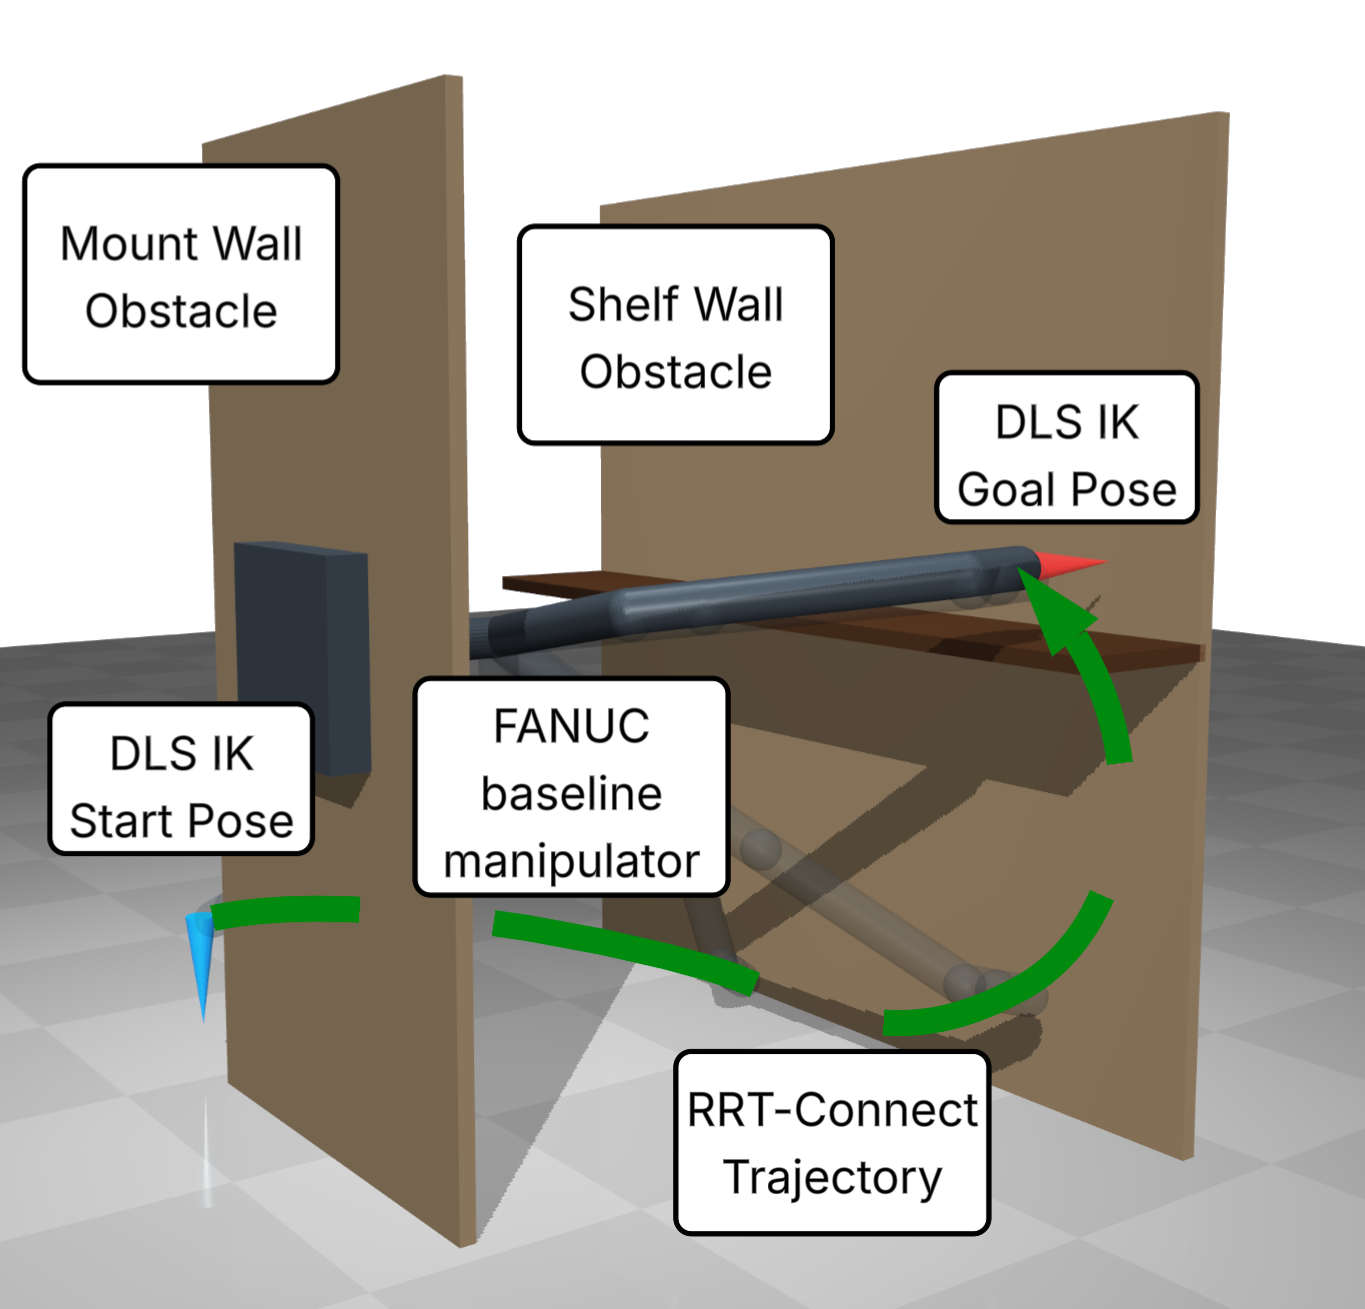
\includegraphics[width=\textwidth]{wallMountTask1.png}
            \caption{Task 1: Mount Wall to Shelf}
            \label{fig:wallMount_1}
        \end{subfigure}
        \hfill
        \begin{subfigure}[b]{0.45\columnwidth}
            \centering
            
\includegraphics[width=\textwidth]{wallMountTask2.png}
            \caption{Task 2: Shelf to Mount Wall}
            \label{fig:wallMount_2}
        \end{subfigure}
        \caption{\textbf{Wall Mount task evaluation.} The manipulator, mounted horizontally on the near wall, must navigate to and from the opposing shelf. Faded overlays represent the RRT-generated trajectory. This configuration evaluates a morphology's ability to resist gravity in atypical base orientations while navigating constrained pick-and-place trajectories.}
        \label{fig:wallMountTask}
    \end{figure}

    \item \textbf{Wall Mount Task}: The robot is mounted on the middle of a wall facing an opposing wall with a shelf mounted in the middle. One start pose is to the side of the mount wall facing down and the corresponding goal pose is on top of the shelf facing toward that wall.
    The other set is the opposite where the start pose is on the shelf facing the wall and the goal is to the side facing down (Figure \ref{fig:wallMountTask}).

    \begin{figure}[tb]
        \centering
        \begin{subfigure}[b]{0.45\columnwidth}
            \centering
            
\includegraphics[width=\textwidth]{shelfTask1.png}
            \caption{Task 1: Top to Bottom}
            \label{fig:shelfTask_1}
        \end{subfigure}
        \hfill
        \begin{subfigure}[b]{0.45\columnwidth}
            \centering
            
\includegraphics[width=\textwidth]{shelfTask2.png}
            \caption{Task 2: Bottom to Top}
            \label{fig:shelfTask_2}
        \end{subfigure}
        \caption{\textbf{Shelf task evaluation.} The manipulator navigates around a floating shelf obstacle, moving from a start pose (blue marker) to a goal pose (red marker). Transparent models illustrate the intermediate joint-space trajectory, concluding at the opaque target configuration. This task specifically tests the morphology's capability to maneuver through vertically constrained spaces and perform complex over-and-under reaching motions typical in industrial pick-and-place operations.}
        \label{fig:shelfTask}
    \end{figure}

    \item \textbf{Shelf Task}: A single shelf obstacle is placed off to the side of the robot at 0.3m height.
    There are two sets of start and goal poses alternately above and below the shelf all facing in the positive x direction (Figure \ref{fig:shelfTask}).

    \begin{figure}[tb]
        \centering
        
\includegraphics[width=0.45\columnwidth]{outreachTask.png}
        \caption{\textbf{Near-Base Outreach task evaluation.} The manipulator extends from a configuration near its base (blue marker) to a distant target coordinate (red marker). Transparent overlays depict the collision-free joint-space trajectory generated by RRT-Connect, terminating at the opaque goal configuration. This obstacle-free environment specifically isolates and evaluates a morphology's maximum functional reach and extension efficiency.}
        \label{fig:outreachTask}
    \end{figure}

    \item \textbf{Outreach Task}: There are no obstacles in this task, the robot is on an open floor, the start pose is near the base facing out and the goal pose is out near the limits of reach for the baseline models (Figure \ref{fig:outreachTask}).

    \begin{figure}[tb]
        \centering
        \begin{subfigure}[b]{0.45\columnwidth}
            \centering
            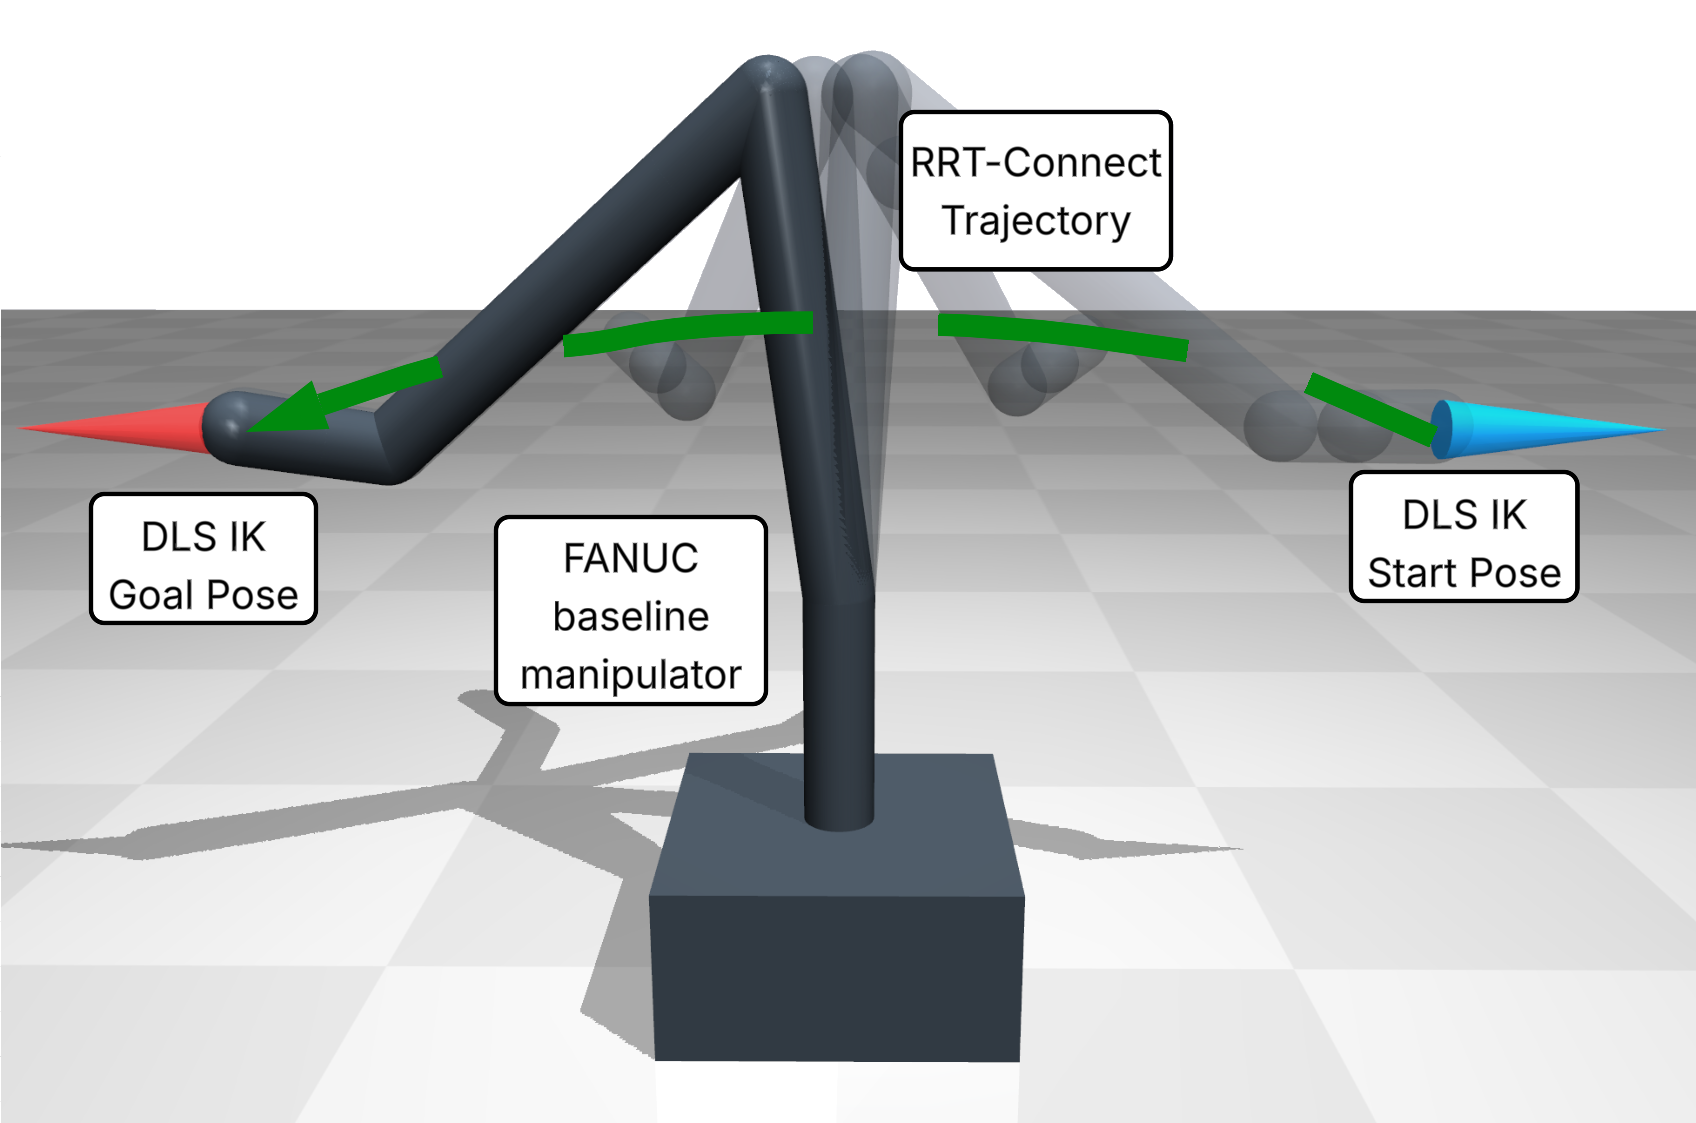
\includegraphics[width=\textwidth]{sideToSideTask1.png}
            \caption{Task 1: Left to Right}
            \label{fig:sideToSide_1}
        \end{subfigure}
        \hfill
        \begin{subfigure}[b]{0.45\columnwidth}
            \centering
            
\includegraphics[width=\textwidth]{sideToSideTask2.png}
            \caption{Task 2: Right to Left}
            \label{fig:sideToSide_2}
        \end{subfigure}
        \caption{\textbf{Side-to-Side outreach evaluation.} The manipulator navigates from the start pose (blue marker) to the goal pose (red marker) across the workspace. Faded models illustrate the intermediate trajectory states discovered by RRT-Connect. This task evaluates the morphology's ability to maximize lateral reach and avoid collision with its own base.}
        \label{fig:sideToSideTask}
    \end{figure}

    \item \textbf{Side-to-Side Task}: Similar to Outreach Task in that there are no obstacles and robot is on open floor, there are two sets of start and goal poses that are alternately on either side of and facing away from the robot (Figure \ref{fig:sideToSideTask}).

\end{enumerate}

The appendix contains the specifications for all of the task obstacles and poses.

\section{Metrics}

Performance is evaluated on each of the tasks averaged over 100 runs with fresh noise each time. Each of the reward terms and the total reward is reported for each task and morphology:

\begin{itemize}
    \item Success rate: fraction of valid IK + RRT paths.
    \item Accuracy \(e\) (m and rads).
    \item Path length \(p\) (m).
    \item Energy \(E\) (J).
    \item Manipulability \(\mu\) (min singular value).
    \item Link count \(n\).
\end{itemize}

\section{Implementation and Compute}

Training uses Stable Baselines3 PPO (1M timesteps, single-step episodes) on a 11th Gen Intel i9-11900KF CPU. The environment was vectorized with 24 parallel instances (`SubprocVecEnv`). Full hyperparameters are in Table~\ref{tab:hyperparams}.

\begin{table}[H]
\caption{PPO Hyperparameters}
\label{tab:hyperparams}
\centering
\begin{tabular}{ll}
\hline
\textbf{Parameter} & \textbf{Value} \\
\hline
Learning rate & 0.001 \\
Horizon (\(n_\text{steps}\)) & 256 \\
Batch size & 512 \\
Epochs per update & 4 \\
Discount factor (\(\gamma\)) & 0.98 \\
Clip ratio (\(\epsilon\)) & 0.2 \\
Value loss coefficient (\(\beta\)) & 0.5 \\
Entropy coefficient & 0.0 \\
\hline
\end{tabular}
\end{table}

\chapter{Results}

Each optimized morphology \(\theta^*\) found by PMorph was compared against the baseline FANUC and Panda across 100 runs in each task.
The average total reward and individual reward terms are reported in Table~\ref{tab:full_results} for each task and morphology, along with the success rate, path length, energy, manipulability, and link count.

\begin{table*}[tbp]
    \centering
    \caption{Performance Metrics Across All Tasks and Morphologies (Averaged over 100 runs)}
    \label{tab:full_results}
    \resizebox{\textwidth}{!}{
        \begin{tabular}{llccccccc}
            \toprule
            \textbf{Task} & \textbf{Model} & \textbf{Links ($n$)} & \textbf{Success (\%)} & \textbf{Pos Err (m)} & \textbf{Rot Err (rad)} & \textbf{Path Len (m)} & \textbf{Energy (J)} & \textbf{Manip. ($\mu$)} \\
            \midrule
            \multirow{5}{*}{\textbf{Container}} 
            & PPO & 7 & 0.0 & 0.039 & 0.279 & $\infty$ & $\infty$ & 0.000 \\
            & SAC & 2 & 21.5 & 0.086 & 0.433 & 1.600 & 31.87 & 0.000 \\
            & CMA-ES & 2 & 3.5 & 0.085 & 0.420 & 1.541 & 31.40 & 0.000 \\
            & FANUC & 6 & 0.0 & 0.032 & 0.474 & $\infty$ & $\infty$ & 0.185 \\
            & Panda & 7 & 55.0 & 0.001 & 0.312 & 2.055 & 36898.65 & 0.224 \\
            \midrule
            \multirow{5}{*}{\textbf{Outreach}} 
            & PPO & 2 & 0.0 & 0.220 & 0.031 & $\infty$ & $\infty$ & 0.000 \\
            & SAC & 2 & 92.0 & 0.050 & 1.380 & 0.521 & 24.22 & 0.000 \\
            & CMA-ES & 4 & 100.0 & 0.011 & 0.042 & 0.554 & 46.29 & 0.000 \\
            & FANUC & 6 & 0.0 & 0.003 & 0.406 & $\infty$ & $\infty$ & 0.144 \\
            & Panda & 7 & 100.0 & 0.001 & 0.360 & 2.072 & 337.13 & 0.220 \\
            \midrule
            \multirow{5}{*}{\textbf{Shelf}} 
            & PPO & 2 & 0.0 & 0.230 & 0.113 & $\infty$ & $\infty$ & 0.000 \\
            & SAC & 2 & 5.0 & 0.113 & 0.586 & 0.840 & 100.36 & 0.000 \\
            & CMA-ES & 4 & 74.5 & 0.048 & 0.751 & 4.025 & 265.16 & 0.000 \\
            & FANUC & 6 & 0.0 & 0.064 & 0.659 & $\infty$ & $\infty$ & 0.171 \\
            & Panda & 7 & 100.0 & 0.002 & 0.332 & 2.828 & 10718.82 & 0.198 \\
            \midrule
            \multirow{5}{*}{\textbf{Side-to-Side}} 
            & PPO & 2 & 100.0 & 0.029 & 0.026 & 0.987 & 23.50 & 0.000 \\
            & SAC & 2 & 100.0 & 0.028 & 0.026 & 0.989 & 23.49 & 0.000 \\
            & CMA-ES & 3 & 100.0 & 0.010 & 0.031 & 1.005 & 31.31 & 0.000 \\
            & FANUC & 6 & 0.0 & 0.002 & 0.375 & $\infty$ & $\infty$ & 0.171 \\
            & Panda & 7 & 100.0 & 0.002 & 0.413 & 2.331 & 4669.10 & 0.157 \\
            \midrule
            \multirow{5}{*}{\textbf{Wall Mount}} 
            & PPO & 2 & 0.0 & 0.384 & 0.090 & $\infty$ & $\infty$ & 0.000 \\
            & SAC & 2 & 50.0 & 0.077 & 1.096 & 1.827 & 37.29 & 0.000 \\
            & CMA-ES & 2 & 50.0 & 0.077 & 1.098 & 1.870 & 46.40 & 0.000 \\
            & FANUC & 6 & 0.0 & 0.070 & 1.594 & $\infty$ & $\infty$ & 0.116 \\
            & Panda & 7 & 37.0 & 0.024 & 1.767 & 3.056 & 257456.71 & 0.189 \\
            \bottomrule
        \end{tabular}
    }
\end{table*}

\section{Energy Efficiency}

The most prominent result across all successful evaluations is the stark contrast in energy consumption between the 7-DOF baseline Panda and the optimized morphologies. The generated morphologies achieved massive energy reductions across all tasks. For example, in the Side-to-Side task, the Panda consumed 4669.10 J, whereas the PPO and SAC generated morphologies consumed only 23.50 J and 23.49 J, respectively. 

This trend is consistent across all tasks where the Panda achieved success, reaching an extreme energy cost of 257,456.71 J in the Wall Mount task. By contrast, the generated morphologies consistently maintained energy costs below 300 J (ranging from 23.49 J to 265.16 J across all recorded successes), demonstrating that the reduction in mass and optimized link configurations drastically reduce the dynamic effort required to complete the trajectories. Energy data for the FANUC baseline could not be recorded as it failed to find a valid kinematic path in any task.

\section{Task Specialization}

Success rates varied significantly depending on the task constraints and the evaluated model. The baseline FANUC failed to achieve a valid path in any task (0.0\% success). The baseline Panda achieved a 100.0\% success rate in open or moderately constrained environments (Outreach, Shelf, and Side-to-Side) but struggled in highly constrained tasks, achieving only 55.0\% in the Container task and 37.0\% in the Wall Mount task.

The optimized morphologies demonstrated varied specialization capabilities depending on the algorithm and the environment. In the obstacle-free Side-to-Side task, PPO, SAC, and CMA-ES all achieved 100.0\% success rates with positional accuracy comparable to the baseline models. CMA-ES also achieved a 100.0\% success rate in the Outreach task. However, in heavily constrained environments like the Container task, the currently evaluated optimized models (SAC and CMA-ES) struggled, achieving only 21.5\% and 3.5\% success rates, respectively. These failures were coupled with higher positional and rotational errors compared to the successful Panda trajectories.

\section{Simplicity}

The optimization framework consistently converged on simpler morphologies compared to the 6-DOF and 7-DOF baselines. Across all tasks, the generated arms reduced the total number of links to between two and four. Notably, both PPO and SAC consistently converged on minimum-complexity 2-link manipulators in the evaluated tasks.

While this simplicity is the primary driver of the observed energy efficiency, it necessitates a trade-off with manipulability and kinematic accuracy. The manipulability index ($\mu$) for all generated morphologies dropped to zero, indicating that the reduced-DOF arms frequently operate at or near kinematic singularities to complete their tasks, unlike the highly redundant baseline models.

\begin{figure}[htbp]
    \centering
    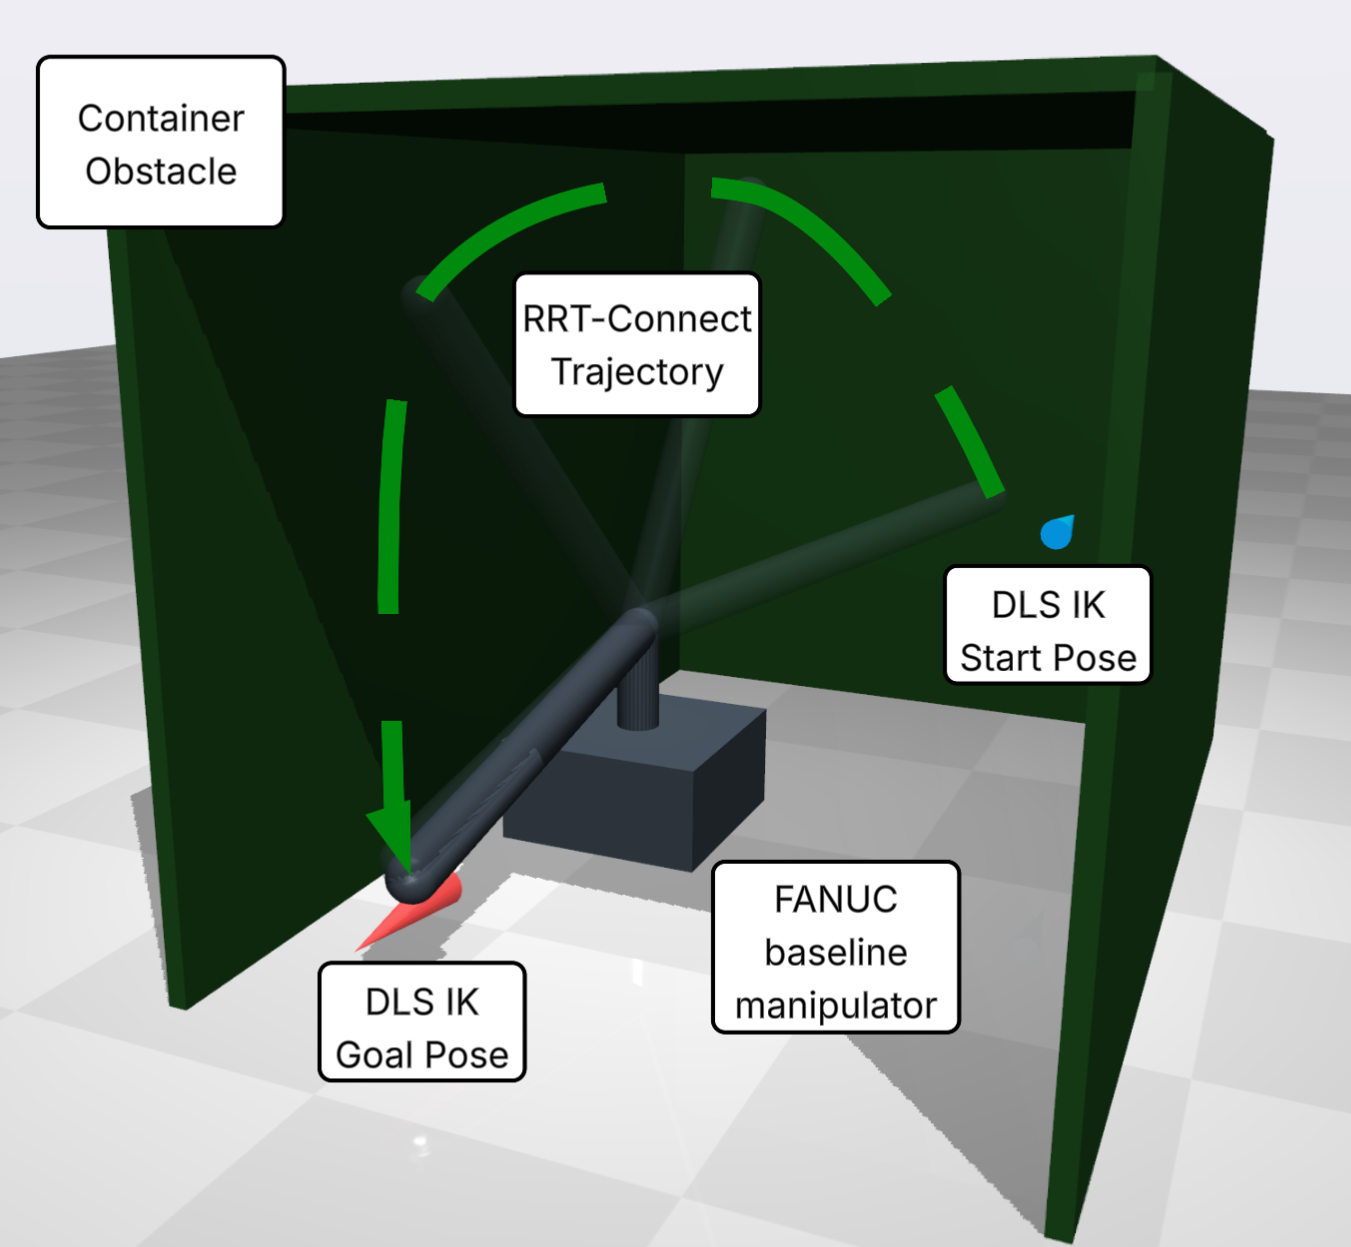
\includegraphics[width=0.9\columnwidth]{sacContainerArm.png}
    \caption{\textbf{SAC-generated Container Task Morphology.} The SAC-generated morphology is shown with a trajectory in the container task. The morphology is simple with 2 links, one z-hinge that's 0.1179m and one y-hinge that's 0.5151m. The manipulator is not quite long enough to reach the start position and significantly off the orientation, but appears right on the goal pose.}
    \label{fig:sacContainerArm}
\end{figure}

Figure \ref{fig:sacContainerArm} illustrates this trade-off using the SAC-generated morphology for the Container task. The morphology is significantly simpler than the generic baseline arms, comprising only two links (one 0.1179m z-hinge and one 0.5151m y-hinge). However, as reflected in the higher error rates in Table \ref{tab:full_results}, this simplicity results in lower accuracy; the manipulator is not quite long enough to accurately reach the start position and exhibits significant orientation error, despite successfully aligning with the goal pose.

\chapter{Conclusion}

This research presented PMorph, a framework designed to address the inefficiencies of generalized industrial robotic manipulators through task-specialized morphology optimization. The results clearly demonstrate that in unconstrained or moderately constrained environments, Reinforcement Learning (specifically PPO, SAC, and CMA-ES) can successfully generate highly energy-efficient, simplified manipulators. By reducing unnecessary degrees of freedom, the optimized models achieved drastic energy reductions while maintaining positional accuracy comparable to industry-standard 6-DOF and 7-DOF arms. 

However, a critical limitation emerged during the evaluation of highly constrained environments. While the framework showed initial promise, the reliance on a simple kinematic path planner created a performance bottleneck as task complexity and obstacle density increased. The planner frequently failed to find valid trajectories for higher-DOF morphologies within the given constraints. Consequently, the optimization agents became biased toward selecting simpler, lower-DOF arms; these simpler morphologies could consistently find viable paths to satisfy the success metric, but lacked the kinematic flexibility to score highly in accuracy or manipulability. 

Ultimately, this study proves that morphological co-optimization is a viable path toward simpler, more efficient industrial robotics. Future work should focus on integrating more sophisticated, dynamically-aware path planners or co-optimizing the control policy alongside the physical morphology. Addressing this planner bottleneck will prevent the optimization agent from defaulting to overly simple designs, unlocking the framework's full potential to generate highly specialized, dexterous manipulators for complex workspaces.
%%%%%%%%%%%%%%%%%%%%%%%%%%%%%%%%%%%%%%%%%%%%%%%%%%%%%%%%%%%%%%%%%%%%%%%%%%%%%%%%

\bibliographystyle{plain}
\nocite{*}		
\bibliography{references}	

%%%%%%%%%%%%%%%%%%%%%%%%%%%%%%%%%%%%%%%%%%%%%%%%%%%%%%%%%%%%%%%%%%%%%%%%%%%%%%%%

\appendix

\chapter{Task Specifications}

\begin{table}[H]
    \centering
    \caption{Container Task Poses}
    \label{tab:containerPoses}
    \begin{tabular}{lll}
    \hline
    \textbf{Name} & \textbf{Position} & \textbf{Quaternion} \\
    \hline
    Start 1 & [-0.45, 0.0, 0.2] & [0.7071, 0, -0.7071, 0] \\
    Goal 1 & [0.45, 0.4, 0.3] & [0.7071, 0, 0.7071, 0] \\
    Start 2 & [-0.45, 0.4, 0.3] & [0.7071, 0, -0.7071, 0] \\
    Goal 2 & [0.45, 0.0, 0.1] & [0.7071, 0, 0.7071, 0] \\
    \hline
    \end{tabular}
\end{table}

\begin{table}[H]
    \centering
    \caption{Container Task Obstacles}
    \label{tab:containerObstacles}
    \begin{tabular}{lll}
    \hline
    \textbf{Name} & \textbf{Position} & \textbf{Size} \\
    \hline
    Back Wall & [-0.6, 0.2, 0.4] & [0.01, 0.4, 0.4] \\
    Left Wall & [0, -0.2, 0.4] & [0.6, 0.01, 0.4] \\
    Right Wall & [0, 0.6, 0.4] & [0.6, 0.01, 0.4] \\
    Ceiling & [0, 0.2, 0.8] & [0.6, 0.4, 0.01] \\
    \hline
    \end{tabular}
\end{table}

\begin{table}[H]
    \centering
    \caption{Wall Mount Task Poses}
    \label{tab:wallMountPoses}
    \begin{tabular}{lll}
    \hline
    \textbf{Name} & \textbf{Position} & \textbf{Quaternion} \\
    \hline
    Start 1 & [-0.4, -0.2, 0.2] & [0, 1, 0, 0] \\
    Goal 1 & [0.5, 0.4, 0.7] & [0.7071, -0.7071, 0, 0] \\
    Start 2 & [-0.2, 0.4, 0.7] & [0.7071, -0.7071, 0, 0] \\
    Goal 2 & [0.4, -0.2, 0.2] & [0, 1, 0, 0] \\
    \hline
    \end{tabular}
\end{table}

\begin{table}[H]
    \centering
    \caption{Wall Mount Task Obstacles}
    \label{tab:wallMountObstacles}
    \begin{tabular}{lll}
    \hline
    \textbf{Name} & \textbf{Position} & \textbf{Size} \\
    \hline
    Mount Wall & [0, -0.2, 0.6] & [0.3, 0.01, 0.6] \\
    Shelf Wall & [0, 0.6, 0.6] & [0.6, 0.01, 0.6] \\
    Shelf & [0.0, 0.5, 0.6] & [0.6, 0.1, 0.01] \\
    \hline
    \end{tabular}
\end{table}

\begin{table}[H]
    \centering
    \caption{Shelf Task Poses}
    \label{tab:simpleShelfPoses}
    \begin{tabular}{lll}
    \hline
    \textbf{Name} & \textbf{Position} & \textbf{Quaternion} \\
    \hline
    Start 1 & [0.45, -0.1, 0.4] & [0.7071, 0, 0.7071, 0] \\
    Goal 1 & [0.35, -0.3, 0.2] & [0.7071, 0, 0.7071, 0] \\
    Start 2 & [0.35, -0.1, 0.2] & [0.7071, 0, 0.7071, 0] \\
    Goal 2 & [0.45, -0.3, 0.4] & [0.7071, 0, 0.7071, 0] \\
    \hline
    \end{tabular}
\end{table}

\begin{table}[H]
    \centering
    \caption{Shelf Task Obstacles}
    \label{tab:simpleShelfObstacles}
    \begin{tabular}{lll}
    \hline
    \textbf{Name} & \textbf{Position} & \textbf{Size} \\
    \hline
    Shelf & [0.4, -0.2, 0.3] & [0.1, 0.2, 0.01] \\
    \hline
    \end{tabular}
\end{table}

\begin{table}[H]
    \centering
    \caption{Near-Base Outreach Task Poses}
    \label{tab:outreachPoses}
    \begin{tabular}{lll}
    \hline
    \textbf{Name} & \textbf{Position} & \textbf{Quaternion} \\
    \hline
    Start & [0.2, 0.2, 0.12] & [0.7071, 0, 0.7071, 0] \\
    Goal & [0.65, 0.2, 0.12] & [0.7071, 0, 0.7071, 0] \\
    \hline
    \end{tabular}
\end{table}

\begin{table}[H]
    \centering
    \caption{Side-to-Side Task Poses}
    \label{tab:sideToSidePoses}
    \begin{tabular}{lll}
    \hline
    \textbf{Name} & \textbf{Position} & \textbf{Quaternion} \\
    \hline
    Start 1 & [0, -0.4, 0.3] & [0.7071, 0.7071, 0, 0] \\
    Goal 1 & [0, 0.4, 0.3] & [0.7071, -0.7071, 0, 0] \\
    Start 2 & [0, 0.4, 0.4] & [0.7071, -0.7071, 0, 0] \\
    Goal 2 & [0, -0.4, 0.4] & [0.7071, 0.7071, 0, 0] \\
    \hline
    \end{tabular}
\end{table}

\end{document}
